\medskip

\textbf{Partie A}


\begin{enumerate}
	\item  Par lecture graphique :

	\begin{center}
		\begin{tikzpicture}
			\tkzTabInit[lgt=3, espcl=4]{$x$/0.8,variations de $f$/1.5}{0,{$1,5 $}, 5 }
			\tkzTabVar{-/{$-5,5$},+/{$2,4$},-/{$0,35$}}
		\end{tikzpicture}
	\end{center}



	\item La courbe $\mathcal{C}$  semble traverser la tangente au point A et donc  admettre un point d'inflexion au point A.

	\item La fonction $f$ est croissante sur l'intervalle $[0~;~1,5[$ puis décroissante sur l'intervalle $]1,5~;~5]$, sa dérivée est donc positive puis négative. La courbe représentant la dérivée $f'$ de $f$ est donc la courbe $\mathcal{C}_2$.

	La fonction $f$ est concave sur $[0~;~2,5[$ puis convexe sur $]2,5~;~5]$, sa dérivée seconde est donc négative puis positive. La courbe représentant la dérivée seconde $f''$ de $f$ est donc la courbe $\mathcal{C}_1$.

	\item Si $F$  est une primitive de $f$, on aura donc $f = F'$ et $f'= F''$.

$f$ est négative sur $[0~;~0,5[$ puis positive, une primitive est donc décroissante sur $[0~;~0,5[$ puis croissante : ce n'est pas le cas (c'est même exactement le contraire) de la fonction représentée par $\mathcal{C}_3$.

$\mathcal{C}_3$ n'est donc pas la représentation graphique d'une primitive de la fonction $f$.




\end{enumerate}

\textbf{Partie B}


\begin{enumerate}
	\item
	\begin{enumerate}
		\item  $f$ est de la forme $u\times v$ avec $u(x)=4x-2$ et $v(x)=\e^{-x+1}$.

		On a donc $u'(x)= 4$ et $v'(x)=-1 \times \e^{-x+1}$.

		$f'= u'v + v'u$ donc, pour tout réel $x$ positif :

		 $f'(x) = 4 \times \e^{-x+1} -1 \times \e^{-x+1} \times (4x-2)= (4-4x+2)\e^{-x+1} = (-4x+6)\e^{-x+1}$.

		\item  Déterminons le signe de $-4x+6$ : \quad $\begin{aligned}[t] -4x+6 >0 &\iff  6 > 4x \\
		&\iff \dfrac{3}{2}>x\end{aligned}$

		les images pertinentes sont : \quad
		$f(0)= (4\times 0 -2) \e ^{-0+1}= -2\e$

		et \quad
		$f\left( \dfrac{3}{2}\right)=  \left(4 \times \dfrac{3}{2}-2\right)\e^{-\frac{3}{2}+1}=4\e^{-\frac{1}{2}}$ \quad (la limite en $+\infty$ est admise).

		\emph{Remarque :} On a $-2\e \approx -5,43$, ce qui confirme la lecture graphique de la \textbf{partie A} \linebreak et $ f\left(\dfrac{3}{2}\right)\approx 2,43 $, là aussi, conforme.


		On a donc le tableau :

		\begin{center}
			\begin{tikzpicture}
				\tkzTabInit[lgt=3]{$x$/0.8,signe de $-4x+6$/0.8,signe de $\e^{-x+1}$/0.8,signe de $f'(x)$/0.8,variations de $f$/2}{0,$\dfrac{3}{2}$,$+\infty$}
				\tkzTabLine{,+,z,-}
				\tkzTabLine{,+,t,+}
				\tkzTabLine{,+,z,-}
				\tkzTabVar{-/$-2\e$,+/$4\e^{-\frac{1}{2}}$,-/0}
			\end{tikzpicture}
		\end{center}


		\item  Pour tout réel $x$ positif on a :

		$f''(x)= -4 \times \e^{-x+1} -1 \times \e^{-x+1} \times (-4x+6)= (-4+4x-6)\e^{-x+1}= (4x-10)\e^{-x+1}$


		Déterminons le signe de  $4x-10$ :\quad $\begin{aligned}[t] 4x-10 >0 &\iff  4x > 10 \\
		&\iff x>\dfrac{5}{2}\end{aligned}$

		\begin{center}
			\begin{tikzpicture}
				\tkzTabInit[lgt=3]{$x$/0.8,signe de $4x-10$/0.8,signe de $\e^{-x+1}$/0.8,signe de $f''(x)$/0.8}{0,$\dfrac{5}{2}$,$+\infty$}
				\tkzTabLine{,-,z,+}
				\tkzTabLine{,+,t,+}
				\tkzTabLine{,-,z,+}
			\end{tikzpicture}
		\end{center}

		La fonction $f$ est donc concave sur $\left[0~;~\dfrac{5}{2}\right]$ et convexe sur $\left[\dfrac{5}{2}~;~+\infty\right[$.

		Le point A, d'abscisse  $\dfrac{5}{2}$ est un point d'inflexion de la courbe représentative de $f$.

		\end{enumerate}
	\item

	\begin{enumerate}
		\item  Soit $F$ la fonction définie sur $[0~;~+\infty[$ par $F(x)=(ax+b)\e^{-x+1}$ avec  $a$ et $b$ deux nombres réels.

		$F$  est dérivable sur $[0~;~+\infty[$ comme produit de fonctions dérivables sur $[0~;~+\infty[$.

		Pour tout réel $x$ positif on a :

		$F'(x)= 1 \times \e^{-x+1} - \times \e^{-x+1} \times (ax+b)= (a-ax-b)\e^{-x+1}= (-ax-b+a)\e^{-x+1}$

		$\begin{aligned} F\text{ est une primitive de }f &\iff F'=f\\
		&\iff \forall x \in \R^+ \quad  (-ax-b+a)\e^{-x+1}= (4x-2)\e^{-x+1} \\
		&\iff \forall x \in \R^+ \quad (-ax-b+a)= (4x-2) \quad \text{ car } \quad \e^{-x+1}>0 \\
		&\iff \begin{cases} -a=4 \\ a-b=-2 \end{cases} \quad\text{par identification des coefficients}\\
		&\iff \begin{cases} a=- 4 \\ b=a+2=-4+2=-2 \end{cases}\end{aligned}$

		$F(x)=(-4x-2)\e^{-x+1}$ est une primitive de $f$ sur $[0~;~+\infty[$.

		\item  $\displaystyle  I = \int_{\frac{3}{2}}^8 f(x) \mathrm{d} x = \Big[(-4x-2)\e^{-x+1} \Big]_{\frac{3}{2}}^8
		= (-4\times 8-2)\e^{-8+1} - \left(-4\times \dfrac{3}{2}-2\right)\e^{-\frac{3}{2}+1} = -34\e^{-7}+ 8\e^{-\frac{1}{2}}$

$I \approx 4,821$ soit $4,82$ à $10^{-2}$ près.

	\end{enumerate}

	\item
	\begin{enumerate}
	\item  La hauteur du point de départ est égale à $f\left(\dfrac{3}{2}\right)= 4\e^{-\frac{1}{2}} \approx 2,426$

soit $2,43\,\rm{m}$ au centimètre près.

	\item L'aire, en unité d'aire,  est égale à l'intégrale $I$ calculée à la question \textbf{3.}

L'unité est le mètre, une unité d'aire est donc égale à $\np[m^2]{1}$.

On veut donc couvrir une surface de : \quad $\dfrac{75}{100} \times 4,82 \, \rm{m}^2$ soit environ $3,62 \,\rm{m}^2$.

De plus : $\dfrac{3,62}{0,8} \approx 4,525$

Il faudra donc 5 bombes de peinture pour réaliser cette œuvre.
	\end{enumerate}
\end{enumerate}
\medskip
